\subsection{Порядок байт}

\begin{frame}
	\tableofcontents[currentsection,currentsubsection]
\end{frame}

\begin{frame}{Играем в игру}
	Напоминание: порядок бит в байте мы из программы никак не определим, на картинке рисуем слева старшие, справа младшие.

	Порядок байт в памяти "--- слева меньшие адреса, справа большие.

	\begin{center}
		\pause
		\begin{tabular}{|c|c|c|c|l|}
			\hline
			\multicolumn{4}{|c|}{Адрес} & Значение \\
			 & 2 & 3 & & \\\hline
			\dots & \t{0000 0001} & \t{0000 0011} & \dots & \pause 259 \\\noalign{\pause}
			\dots & \t{0000 0001} & \t{0000 0011} & \dots & \pause 769 \\
			\hline
		\end{tabular}
		\pause
	\end{center}

	\begin{itemize}
		\item
			В каком порядке идут байты в памяти?
			Они же тоже бывают старшие и младшие.
		\item
			Как договорились "--- так и идут.
			Договариваются по-разному на разных процессорах и в разных протоколах.
		\item
			Свойство <<порядок байт>> называется endianness.
	\end{itemize}
\end{frame}

\begin{frame}

	\begin{center}
		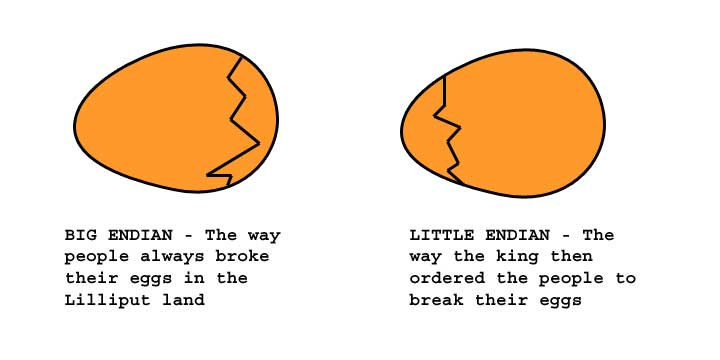
\includegraphics[scale=0.3]{eggs.jpg}
	\end{center}

	Есть два клана: little-endian (остроконечники) и big-endian (тупоконечники).
	По-русски всегда используют английские термины.
\end{frame}

\begin{frame}{Big-endian}
	Используется в низкоуровневых сетевых протоколах (TCP) и процессорах Atmel AVR (ATmega и прочие).

	Младший байт имеет больший адрес.
	Читается просто:
	\begin{center}
		\begin{tabular}{|c|c|c|c|l|}
			\hline
			\multicolumn{4}{|c|}{Адрес} & Значение \\
			& 2 & 3 & & \\\hline
			\dots & \t{0000 0001} & \t{0000 0011} & \dots & $\t{0000~00\textbf{01}~0000~00\textbf{11}}_2=259_{10}$ \\
			\hline
		\end{tabular}
	\end{center}

	Надо очень аккуратно помнить адрес и размер числа:
	\begin{center}
		\begin{tabular}{|c|c|c|l|}
			\hline
			\multicolumn{3}{|c|}{Адрес} & Значение \\
			& 2 & & \\\hline
			\dots & \t{0000 0001} & \dots & $\t{0000 0001}_2=1_{10}$ \\
			\hline
		\end{tabular}
	\end{center}
\end{frame}

\begin{frame}{Little-endian}
	Используется в x86: <<младший байт имеет меньший адрес>>.

	Читается хуже:
	\begin{center}
		\begin{tabular}{|c|c|c|c|l|}
			\hline
			\multicolumn{4}{|c|}{Адрес} & Значение \\
			& 2 & 3 & & \\\hline
			\dots & \t{0000 0001} & \t{0000 0011} & \dots & $\t{0000~00\textbf{11}~0000~00\textbf{01}}_2=769_{10}$ \\
			\hline
		\end{tabular}
	\end{center}
	Если только мы не Intel и не пишем к этому документацию:
	\begin{center}
		\begin{tabular}{|c|c|c|c|l|}
			\hline
			\multicolumn{4}{|c|}{Адрес} & Значение \\
			& \textbf{3} & \textbf{2} & & \\\hline
			\dots & \t{0000 0011} & \t{0000 0001} & \dots & $\t{0000~0011~0000~0001}_2=769_{10}$ \\
			\hline
		\end{tabular}
	\end{center}
	Они у себя всё пишут от старших к младшим: байты с меньшими адресами справа, младшие биты справа.
\end{frame}

\begin{frame}{Особенности Little-endian-1}
	Можно почти безболезненно конвертировать между типами:
	\begin{center}
		\begin{tabular}{|c|c|c|c|r|l|}
			\hline
			\multicolumn{4}{|c|}{Адрес} & \multicolumn{2}{|c|}{Значение} \\
			& 2 & 3 & & & \\\hline
			\dots & \t{0000 0011} & \t{0000 0001} & \dots & $\t{0000~0001~0000~0011}_2$ & $259_{10}$ \\
			\dots & \t{0000 0011} & \dots         & \dots & $\t{0000~0001}_2$           & $3_{10}$ \\
			\dots & \t{0000 0101} & \t{0000 0000} & \dots & $\t{0000~0000~0000~0101}_2$ & $5_{10}$ \\
			\dots & \t{0000 0101} & \dots         & \dots & $\t{0000~0101}_2$           & $5_{10}$ \\
			\dots & \t{1111 0011} & \t{0000 0000} & \dots & $\t{0000~0000~1111~0011}_2$ & $243_{10}$ \\
			\dots & \t{1111 0011} & \dots         & \dots & $\t{1111~0011}_2$           & $243_{10}$ \\
			\dots & \t{1111 0011} & \dots         & \dots & $\t{1111~0011}_2$           & $-13_{10}$ \\
			\dots & \t{1111 0011} & \t{1111 1111} & \dots & $\t{1111~1111~1111~0011}_2$ & $-13_{10}$ \\
			\hline
		\end{tabular}
	\end{center}
\end{frame}

\begin{frame}[t]{Особенности Little-endian-2}
	\begin{itemize}
		\item
			Есть проблема со знаком, если мы переходим от меньшего типа к большему.
		\item
			Надо \textit{расширять знак}, если у нас было знаковое число:
			заполнять старшие байты либо нулями, либо единицами (в зависимости от\only<1>{...}\only<2->{ старшего бита в числе}).
	\only<3->{
		\item
			Если число было беззнаковое, то надо старший байт заполнить нулями.
	}
	\end{itemize}

	\only<3->{
	Компиляторы низкоуровневых языков делают это автоматически, когда вы делаете какие-то присваивания.
	Разумеется, надо аккуратно следить за типами, иначе не сделают.

	Замечание: иногда, несмотря на тип \t{int}, какие-то функции могут ожидать в нём на самом деле не число,
	а набор байт в определённом порядке.
	Яркий пример "--- номер порта в работе с сетью на C, функция \t{htons} "--- это оно.
	}
\end{frame}

\begin{frame}{Резюме}
	\begin{enumerate}
		\item
			Целые числа хранятся в двоичной системе счисления.
		\item
			Знаковость числа определяется лишь типом данных.
		\item
			Самый распространённый способ кодирования отрицательных чисел "--- <<дополнительный код>>.
		\item
			В дополнительном коде старший бит отвечает за знак, а арифметика делатеся так же, как и в беззнаковых числах.
		\item
			Операциям сравнения чисел на меньше/больше и делению важно знать, работаем ли мы в дополнительном коде или с беззнаковыми числами.
		\item
			Порядок байт в числах может отличаться даже в разных местах внутри одного приложения.
			Читайте документацию, если работаете с чем-то на уровне байт!
		\item
			Если работаете с little-endian и меняете количество байт в числе "--- позаботьтесь о знаке.
		\item
			Если есть либо дополнительный код, либо переполнения, то важно количество бит/байт в числе.
	\end{enumerate}
\end{frame}
